% \chapter{Některé příkazy balíčku \texttt{thesis}}
% 
% \section{Příkazy pro sazbu veličin a jednotek}
% 
% \begin{table}[!h]
%   \caption[Přehled příkazů]{Přehled příkazů pro matematické prostředí }
%   \begin{center}
%   	\small
% 	  \begin{tabular}{|c|c|c|c|}
% 	    \hline
% 	    Příkaz    						& Příklad 					& Zdroj příkladu  							& Význam  \\
% 	    \hline\hline
% 	    \verb|\textind{...}|	& $\beta_\textind{max}$ 	& \verb|$\beta_\textind{max}$|	& textový index \\
% 	    \hline
% 	    \verb|\const{...}| 		& $\const{U}_\textind{in}$ 				& \verb|$\const{U}_\textind{in}$|		& konstantní veličina \\
% 	    \hline
% 	    \verb|\var{...}| 		& $\var{u}_\textind{in}$ & \verb|$\var{u}_\textind{in}$| & proměnná veličina \\
% 	    \hline
% 	    \verb|\complex{...}| 	& $\complex{u}_\textind{in}$ & \verb|$\complex{u}_\textind{in}$| & komplexní veličina \\
% 	    \hline
% 	    \verb|\vect{...}| 		& $\vect{y}$ 						& \verb|$\vect{y}$| & vektor \\
% 	    \hline
% 	    \verb|\mat{...}| 	& $\mat{Z}$ 						& \verb|$\mat{Z}$| & matice \\
% 	    \hline
% 	    \verb|\unit{...}| 		& $\unit{kV}$ 						& \verb|$\unit{kV}$|\quad či\ \, \verb|\unit{kV}| & jednotka \\
% 	    \hline
% 	  \end{tabular}
%   \end{center}
% \end{table}
% 
% 
% 
% %\newpage
% \section{Příkazy pro sazbu symbolů}
% 
% \begin{itemize}
%   \item
%     \verb|\E|, \verb|\eul| -- sazba Eulerova čísla: $\eul$,
%   \item
%     \verb|\J|, \verb|\jmag|, \verb|\I|, \verb|\imag| -- sazba imaginární jednotky: $\jmag$, $\imag$,
%   \item
%     \verb|\dif| -- sazba diferenciálu: $\dif$,
%   \item
%     \verb|\sinc| -- sazba funkce: $\sinc$,
%   \item
%     \verb|\mikro| -- sazba symbolu mikro stojatým písmem%
% 			\footnote{znak pochází z~balíčku \texttt{textcomp}}: $\mikro$,
% 	\item
% 		\verb|\uppi| -- sazba symbolu $\uppi$
% 			(stojaté řecké pí, na rozdíl od \verb|\pi|, což sází $\pi$).
% \end{itemize}
% %
% Všechny symboly jsou určeny pro matematický mód, vyjma \verb|\mikro|, jenž je\\ použitelný rovněž v~textovém módu.
% %$\upmikro$
% 
% 
% \chapter{Druhá příloha}
% 
% \begin{figure}[!h]
%   \begin{center}
%     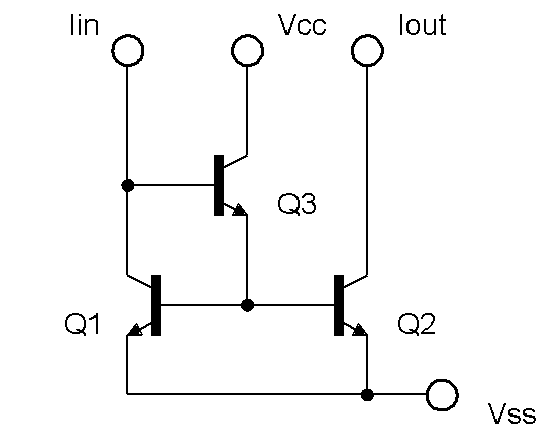
\includegraphics[scale=0.5]{obrazky/ZlepseneWilsonovoZrcadloNPN}
%   \end{center}
%   \caption[Alenčino zrcadlo]{Zlepšené Wilsonovo proudové zrcadlo.}
% \end{figure}
% 
% Pro sazbu vektorových obrázků přímo v~\LaTeX{}u je možné doporučit balíček \href{https://www.ctan.org/pkg/pgf}{\texttt{TikZ}}.
% Příklady sazby je možné najít na \href{http://www.texample.net/tikz/examples/}{\TeX{}ample}.
% Pro vyzkoušení je možné použít programy QTikz nebo TikzEdt.
% 
% 
% 
% 
% \chapter{Příklad sazby zdrojových kódů}
% 
% \section{Balíček \texttt{listings}}
% 
% Pro vysázení zdrojových souborů je možné použít balíček \href{https://www.ctan.org/pkg/listings}{\texttt{listings}}.
% Balíček zavádí nové prostředí \texttt{lstlisting} pro sazbu zdrojových kódů, jako například:
% %
% \begin{lstlisting}[language={[LaTeX]TeX}]
% \section{Balíček lstlistings}
% Pro vysázení zdrojových souborů je možné použít
% 	balíček \href{https://www.ctan.org/pkg/listings}%
% 	{\texttt{listings}}.
% Balíček zavádí nové prostředí \texttt{lstlisting} pro
% 	sazbu zdrojových kódů.
% \end{lstlisting}
% %
% Podporuje množství programovacích jazyků.
% Kód k~vysázení může být načítán přímo ze zdrojových souborů.
% Umožňuje vkládat čísla řádků nebo vypisovat jen vybrané úseky kódu.
% Např.:
% 
% \noindent
% Zkratky jsou sázeny v~prostředí \texttt{acronym}:
% \label{lst:zkratky}
% \lstinputlisting[language={[LaTeX]TeX},nolol,numbers=left, firstnumber=6, firstline=6,lastline=6]{text/zkratky.tex}
% %
% Šířka textu volitelného parametru \verb|KolikMista| udává šířku prvního sloupce se zkratkami.
% Proto by měla být zadávána nejdelší zkratka nebo symbol.
% Příklad definice zkratky \acs{symfvz} je na výpisu \ref{lst:symfvz}.
% 
% \shorthandoff{-}
% \lstinputlisting[language={[LaTeX]TeX},frame=single,caption={Ukázka sazby zkratek},label=lst:symfvz,numbers=left,linerange={bsymfvz-\%\%\%\ esymfvz},includerangemarker=false]{text/zkratky.tex}
% \shorthandon{-}
% 
% \noindent
% Ukončení seznamu je provedeno ukončením prostředí:
% \lstinputlisting[language={[LaTeX]TeX},nolol,numbers=left,firstnumber=26,linerange=26]{text/zkratky.tex}
% 
% \vspace{\fill}
% 
% \noindent
% {\bf Poznámka k~výpisům s~použitím volby jazyka \verb|czech| nebo \verb|slovak|:}\newline
% Pokud Váš zdrojový kód obsahuje znak spojovníku \verb|-|, pak překlad může skončit chybou.
% Ta je způsobená tím, že znak \verb|-| je v~českém nebo slovenském nastavení balíčku \verb|babel| tzv.\ aktivním znakem.
% Přepněte znak \verb|-| na neaktivní příkazem \verb|\shorthandoff{-}| těsně před výpisem a hned za ním jej vraťte na aktivní příkazem \verb|\shorthandon{-}|.
% Podobně jako to je ukázáno ve zdrojovém kódu šablony.
% 
% 
% \clearpage
% 
% %\section{Výpis kódu prostředí Matlab}
% Na výpisu \ref{lst:priklad.vypis.kodu.Matlab} naleznete příklad kódu pro Matlab, na výpisu \ref{lst:priklad.vypis.kodu.C} zase pro jazyk~C.
% 
% \lstnewenvironment{matlab}[1][]{%
% \iflanguage{czech}{\shorthandoff{-}}{}%
% \iflanguage{slovak}{\shorthandoff{-}}{}%
% \lstset{language=Matlab,numbers=left,#1}%
% }{%
% \iflanguage{slovak}{\shorthandon{-}}{}%
% \iflanguage{czech}{\shorthandon{-}}{}%
% }
% 
% \begin{matlab}[frame=single,float=htbp,caption={Příklad Schur-Cohnova testu stability v~prostředí Matlab.},label=lst:priklad.vypis.kodu.Matlab,numberstyle=\scriptsize, numbersep=7pt]
% %% Priklad testovani stability filtru
% 
% % koeficienty polynomu ve jmenovateli
% a = [ 5, 11.2, 5.44, -0.384, -2.3552, -1.2288];
% disp( 'Polynom:'); disp(poly2str( a, 'z'))
% 
% disp('Kontrola pomoci korenu polynomu:');
% zx = roots( a);
% if( all( abs( zx) < 1))
%     disp('System je stabilni')
% else
%     disp('System je nestabilni nebo na mezi stability');
% end
% 
% disp(' '); disp('Kontrola pomoci Schur-Cohn:');
% ma = zeros( length(a)-1,length(a));
% ma(1,:) = a/a(1);
% for( k = 1:length(a)-2)
%     aa = ma(k,1:end-k+1);
%     bb = fliplr( aa);
%     ma(k+1,1:end-k+1) = (aa-aa(end)*bb)/(1-aa(end)^2);
% end
% 
% if( all( abs( diag( ma.'))))
%     disp('System je stabilni')
% else
%     disp('System je nestabilni nebo na mezi stability');
% end
% \end{matlab}
% 
% \noindent
% \begin{minipage}{\linewidth}
% 
% 
% %\section{Výpis kódu jazyka C}
% 
% \begin{lstlisting}[frame=single,numbers=right,caption={Příklad implementace první kanonické formy v~jazyce C.},label=lst:priklad.vypis.kodu.C,basicstyle=\ttfamily\small, keywordstyle=\color{black}\bfseries\underbar,]
% // první kanonická forma
% short fxdf2t( short coef[][5], short sample)
% {
% 	static int v1[SECTIONS] = {0,0},v2[SECTIONS] = {0,0};
% 	int x, y, accu;
% 	short k;
% 
% 	x = sample;
% 	for( k = 0; k < SECTIONS; k++){
% 		accu = v1[k] >> 1;
% 		y = _sadd( accu, _smpy( coef[k][0], x));
% 		y = _sshl(y, 1) >> 16;
% 
% 		accu = v2[k] >> 1;
% 		accu = _sadd( accu, _smpy( coef[k][1], x));
% 		accu = _sadd( accu, _smpy( coef[k][2], y));
% 		v1[k] = _sshl( accu, 1);
% 
% 		accu = _smpy( coef[k][3], x);
% 		accu = _sadd( accu, _smpy( coef[k][4], y));
% 		v2[k] = _sshl( accu, 1);
% 
% 		x = y;
% 	}
% 	return( y);
% }
% \end{lstlisting}
% \end{minipage}
% 
% 
% 
% 
% 
% 
% 
%  \chapter{Obsah elektronické přílohy}
%  Elektronická příloha je často nedílnou součástí semestrální nebo závěrečné práce.
%  Vkládá se do informačního systému VUT v~Brně ve vhodném formátu (ZIP, PDF\,\dots).
%  
%  Nezapomeňte uvést, co čtenář v~této příloze najde.
%  Je vhodné okomentovat obsah každého adresáře, specifikovat, který soubor obsahuje důležitá nastavení, který soubor je určen ke spuštění, uvést nastavení kompilátoru atd.
%  Také je dobře napsat, v~jaké verzi software byl kód testován (např.\ Matlab 2018b).
%  Pokud bylo cílem práce vytvořit hardwarové zařízení,
%  musí elektronická příloha obsahovat veškeré podklady pro výrobu (např.\ soubory s~návrhem DPS v~Eagle).
%  
%  Pokud je souborů hodně a jsou organizovány ve více složkách, je možné pro výpis adresářové struktury použít balíček \href{https://www.ctan.org/pkg/dirtree}{\texttt{dirtree}}.
%  
%  \bigskip
%  
%  {\small
%  %
%  \dirtree{%.
%  .1 /\DTcomment{kořenový adresář přiloženého archivu}.
%  .2 logo\DTcomment{loga školy a fakulty}.
%  .3 BUT\_abbreviation\_color\_PANTONE\_EN.pdf.
%  .3 BUT\_color\_PANTONE\_EN.pdf.
%  .3 FEEC\_abbreviation\_color\_PANTONE\_EN.pdf.
%  .3 FEKT\_zkratka\_barevne\_PANTONE\_CZ.pdf.
%  .3 UTKO\_color\_PANTONE\_CZ.pdf.
%  .3 UTKO\_color\_PANTONE\_EN.pdf.
%  .3 VUT\_barevne\_PANTONE\_CZ.pdf.
%  .3 VUT\_symbol\_barevne\_PANTONE\_CZ.pdf.
%  .3 VUT\_zkratka\_barevne\_PANTONE\_CZ.pdf.
%  .2 obrazky\DTcomment{ostatní obrázky}.
%  .3 soucastky.png.
%  .3 spoje.png.
%  .3 ZlepseneWilsonovoZrcadloNPN.png.
%  .3 ZlepseneWilsonovoZrcadloPNP.png.
%  .2 pdf\DTcomment{pdf stránky generované informačním systémem}.
%  .3 student-desky.pdf.
%  .3 student-titulka.pdf.
%  .3 student-zadani.pdf.
%  .2 text\DTcomment{zdrojové textové soubory}.
%  .3 literatura.tex.
%  .3 prilohy.tex.
%  .3 reseni.tex.
%  .3 uvod.tex.
%  .3 vysledky.tex.
%  .3 zaver.tex.
%  .3 zkratky.tex.
%  %.2 navod-sablona\_FEKT.pdf\DTcomment{návod na používání šablony}.
%  .2 sablona-obhaj.tex\DTcomment{hlavní soubor pro sazbu prezentace k~obhajobě}.
%  %.2 readme.txt\DTcomment{soubor s~popisem obsahu CD}.
%  .2 sablona-prace.tex\DTcomment{hlavní soubor pro sazbu kvalifikační práce}.
%  .2 thesis.sty\DTcomment{balíček pro sazbu kvalifikačních prací}.
%  }
%  }
%  